\chapter{Introduktion}
Denne rapport gennemgår arbejdet med Øvelse 12 i I4IKN. Den indeholder beskrivelser af den protokol stak der er udviklet i opgaven. Beskrivelserne er delt op i de to lag hvor hoveddelen af arbejdet har været: Link- og Transportlag. \\

Transportlagets overordnede funktion vises på figur \ref{fig:protokolstak}. Her ses hvordan kommunikation bevæger sig fra fra applikationen, igennem transportlaget og videre til linklaget. I linklaget enkodes kommunikationen med den slip protokollen beskrevet i sektion \ref{sec:encoding} hvorefter dataen sendes over den fysiske forbindelse.

\begin{figure}[H]
	\centering
	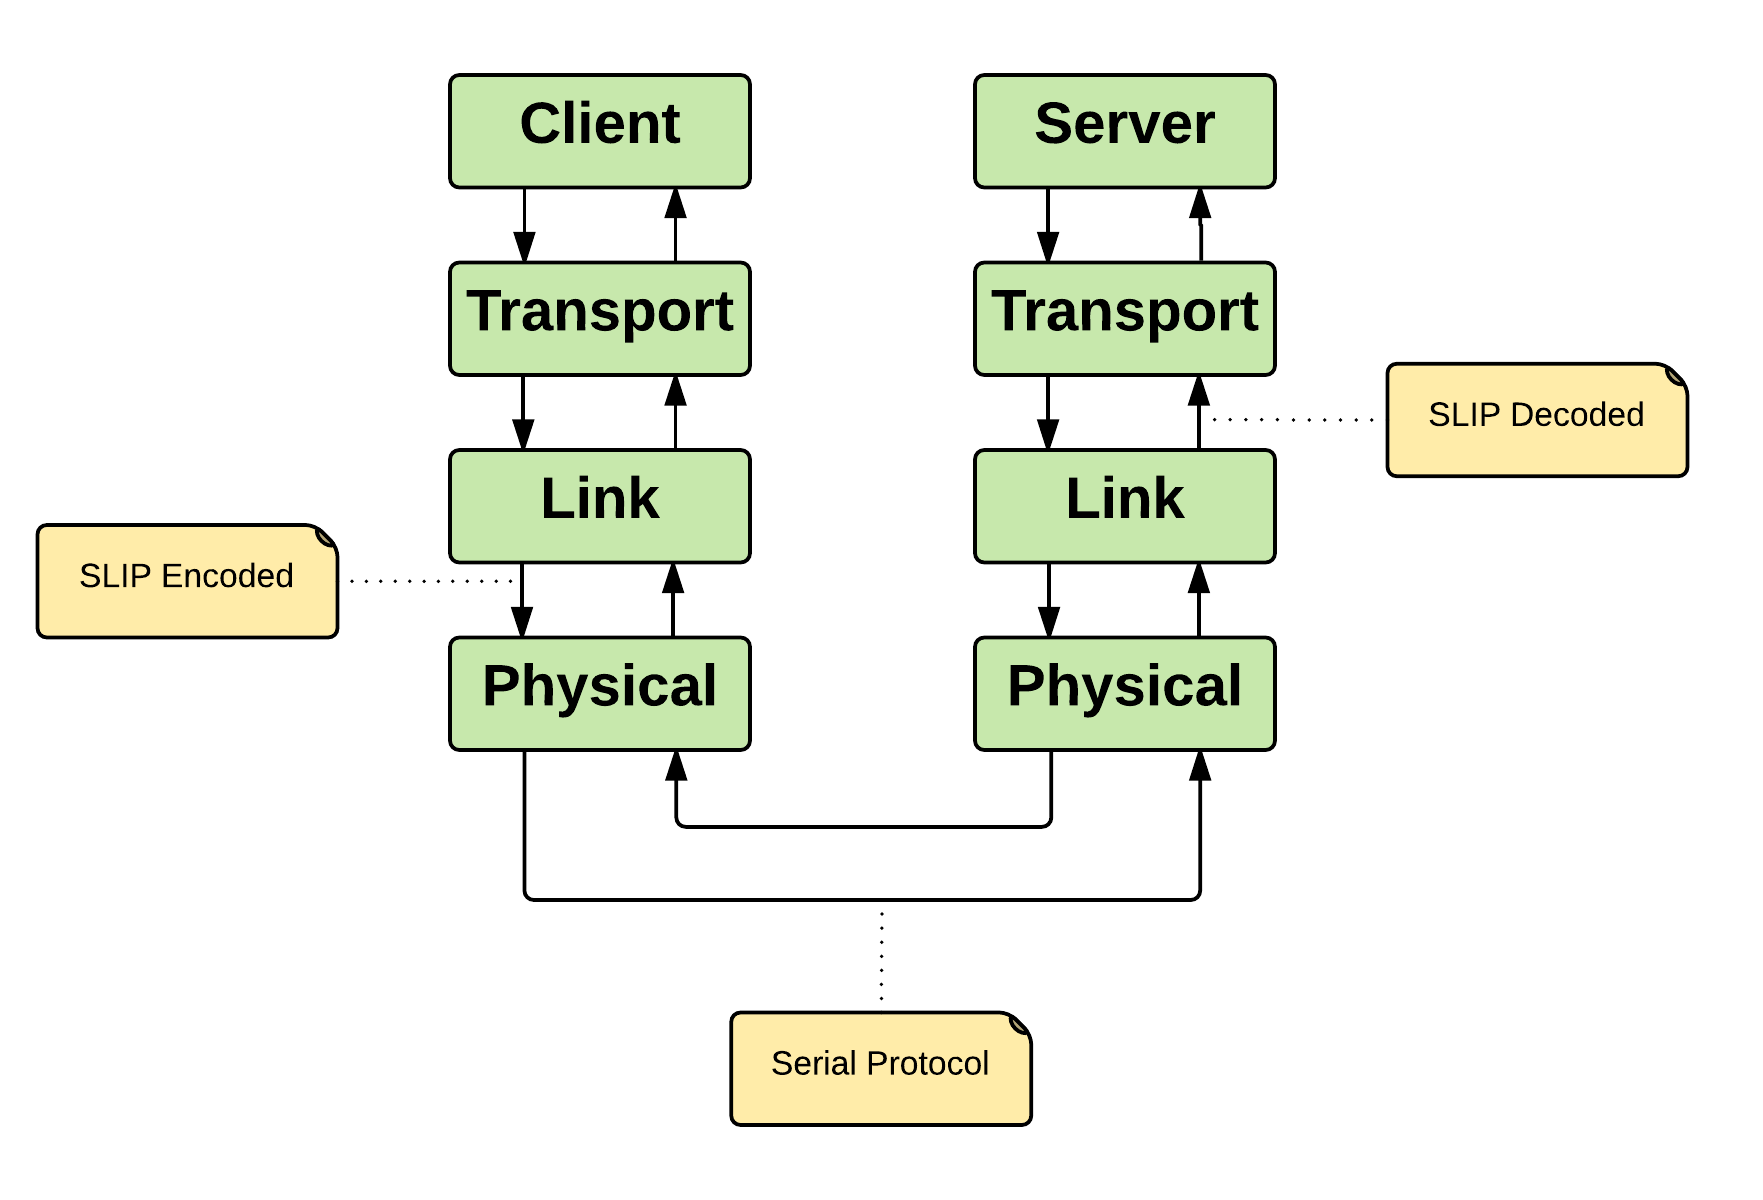
\includegraphics[width=.9\textwidth]{ProtocolStack.png}
	\caption{Generel beskrivelse af protokolstakkens funktion}
	\label{fig:protokolstak}
\end{figure}